\section{Experiments}
\label{experiments}


\subsection{Evaluation Setup}
\label{sec:evaluation_setup}

\paragraph{Benchmark Models.}
We benchmark a diverse set of state-of-the-art (SOTA) multimodal large language models, comprising both leading proprietary models (GPT-5~\cite{OpenAI2025} and Gemini 2.5-Pro~\cite{Gemini2025}) and top-tier open-source models (VideoLLama3~\cite{zhang2025videollama}, Qwen2.5-VL~\cite{bai2025qwen2}, Qwen3-VL~\cite{bai2025qwen2}, and InternVL3.5~\cite{wang2025internvl3}).
To analyze the impact of model capacity, we evaluate variants across model sizes ranging from 7B to 241B parameters.
In total, we comprehensively evaluate eleven models on Spatial4D-Bench.
At the time of evaluation, these models represented the state-of-the-art.
We note that the results reported for proprietary models reflect the versions accessible during our experimental window; as these API-based services are subject to continuous updates by their providers, exact reproducibility may vary over time.
For memory-intensive models (\eg, 241B parameters), we adopt a uniform sampling strategy of $64$ frames from each video to mitigate memory constraints during evaluation following~\cite{Yang_2025_CVPR}.



\paragraph{Evaluation Protocol.}
We conduct all evaluations under a zero-shot setting.
Adhering to the protocol established in~\cite{Yang_2025_CVPR}, we compute the metrics tailored to the distinct answer formats in our Spatial4D-Bench, including Multiple-Choice Answers (MCA) and Numerical Answers (NA).
For MCA tasks, we report  exact matching with possible fuzzy matching.
For NA tasks, we evaluate performance using the Mean Relative Accuracy (MRA).
The MRA measures the model's consistency across a spectrum of error tolerances, calculated as the average satisfaction rate over a set of thresholds $\mathcal{C}$, which is defined as follows:
\begin{equation}
    \mathrm{MRA} = \frac{1}{|\mathcal{C}|}\sum_{\theta \in \mathcal{C} }\mathbbm{1} \left( \frac{\left | \hat{y} - y \right | }{y} < 1 - \theta \right), 
\end{equation}
where $\hat{y}$ and $y$ represent the predicted value and ground truth, respectively.
The threshold set is defined as $\mathcal{C} = \{0.5, 0.55, ... ,0.95\}$, representing a range of strictness levels.



\paragraph{Reference Baselines.}
Similar to~\cite{Yang_2025_CVPR}, to contextualize MLLM performance, we compare against the baselines of: \textit{Human Level Performance} and \textit{Chance Level Baselines (Random and Frequency)}. 
For \textit{Human Level Performance}, we sample 1,000 QA pairs from Spatial4D-Bench as a representative subset and recruited several qualified human evaluators with relevant research background to independently complete the test.
To establish a theoretical ceiling for the performance of human-level 4D spatial intelligence, we report the highest score among human evaluators. 
For \textit{Chance Level (Random)}, we report the expected average accuracy of random selection (MCA only).
For \textit{Chance Level (Frequency)}, we report performance by always selecting the dataset's most frequent answer for each task. This indicates the potential performance gains that could be obtained due to the long-tail distribution of answers or the imbalance in multiple-choice distributions.







\subsection{Main Evaluation Results}
\label{sec:main_results}
We present the main evaluation results in \cref{table:main_eval_18_tasks} and show radar chart visualization of model performance across 18 tasks in \cref{Main_results_radar_plot}.
Our analysis and discussion of the main evaluation results are as follows.


\begin{table}
\centering
\scriptsize
\resizebox{\textwidth}{!}{
\begin{tabular}{llcccccccccccccc}
\toprule
& & & \multicolumn{2}{c}{\textit{Chance Level}} & \multicolumn{2}{c}{\textit{Proprietary Models}} & \multicolumn{9}{c}{\textit{Open-source Models}} \\
\cmidrule(lr){4-5} \cmidrule(lr){6-7} \cmidrule(lr){8-16}
 &  &  & &  & & & \multicolumn{2}{c}{\textbf{Qwen3-VL}} & \multicolumn{3}{c}{\textbf{InternVL3.5}} & \multicolumn{3}{c}{\textbf{Qwen2.5-VL}} & \textbf{VideoLlama3} \\
 \cmidrule(lr){8-9} \cmidrule(lr){10-12} \cmidrule(lr){13-15} \cmidrule(lr){16-16}
\multirow{-2}{*}{\textbf{Category}} & \multirow{-2}{*}{\textbf{Task}} & \multirow{-2}{*}{\textbf{Human}} & \multirow{-2}{*}{\textbf{Rand.}} & \multirow{-2}{*}{\textbf{Freq.}} & \multirow{-2}{*}{\textbf{GPT-5}}  & \multirow{-2}{*}{\textbf{\begin{tabular}[c]{@{}c@{}}Gemini 2.5\\ Pro\end{tabular}}} & \textbf{\tiny 235B-A22B} & \textbf{\tiny 30B-A3B} & \textbf{\tiny 241B-A28B} & \textbf{\tiny 38B} & \textbf{\tiny 8B} & \textbf{\tiny 72B} & \textbf{\tiny 32B} & \textbf{\tiny 7B} & \textbf{\tiny 7B} \\ \midrule
\multirow{4}{*}{Object Understanding} & Object Size & \cellcolor{tabgrey}{74.61} & - & - & 78.64 & 74.14 & 79.76 & \cellcolor{taborange}{80.10} & 62.17 & 65.63 & 47.39 & 65.47 & 62.27 & 35.63 & 33.21 \\
 & Object Attribute & 89.09 & 25.00 & 29.32 & \cellcolor{taborange}{68.71} & 67.25 & \cellcolor{tabgreen}{62.21} & 58.92 & 57.83 & 55.00 & 47.96 & 59.58 & 56.08 & 52.29 & 52.88 \\ 
& Object Counting & \cellcolor{tabgrey}{66.79} & - & - & 54.49 & 32.40 & 64.70 & \cellcolor{taborange}{67.74} & 63.63 & 60.59 & 55.99 & 33.65 & 37.89 & 46.84 & 52.69 \\ 
& Affordance & 81.48 & 25.00 & 28.27 & \cellcolor{taborange}{67.41} & 56.82 & 57.82 & 52.41 & 59.86 & \cellcolor{tabgreen}{63.36} & 49.41 & 54.86 & 51.00 & 40.00 & 33.91 \\ \midrule
\multirow{3}{*}{Scene Understanding} & Room Size & \cellcolor{tabgrey}{55.00} & - & - & 46.56 & 49.19 & 56.65 & \cellcolor{taborange}{67.22} & 47.62 & 55.02 & 50.16 & 39.97 & 50.35 & 39.82 & 28.41 \\
& Scene Classification & 83.33 & 25.00 & 26.11 & \cellcolor{taborange}{75.16} & 65.59 & \cellcolor{tabgreen}{64.38} & 54.72 & 58.06 & 61.18 & 48.40 & 51.81 & 52.32 & 42.71 & 50.86 \\
 & 3D Grounding & 78.85 & 25.00 & 33.90 & \cellcolor{taborange}{70.59} & 70.44 & \cellcolor{tabgreen}{60.88} & 50.55 & 47.35 & 38.09 & 33.86 & 31.14 & 29.41 & 25.96 & 26.99 \\ \midrule
\multirow{3}{*}{\begin{tabular}[l]{@{}l@{}}Spatial Relationship\\Understanding\end{tabular}} & Absolute Distance & 48.08 & - & - & 37.69 & 30.00 & \cellcolor{taborange}{44.52} & 42.20 & 31.80 & 28.51 & 25.89 & 24.90 & 28.15 & 18.93 & 23.84 \\
 & Relative Distance & 71.15 & 25.00 & 30.57 & \cellcolor{taborange}{68.57} & 63.37 & 60.23 & 58.11 & \cellcolor{tabgreen}{62.81} & 55.48 & 48.51 & 44.16 & 45.28 & 38.96 & 41.99 \\
 & Relative Orientation & 69.23 & 25.00 & 25.12 & 49.25 & 42.33 & \cellcolor{taborange}{55.40} & 53.94 & 31.16 & 52.47 & 40.17 & 21.02 & 42.29 & 24.79 & 31.01 \\ \midrule
\multirow{4}{*}{\begin{tabular}[l]{@{}l@{}}Spatiotemporal\\Relationship\\Understanding\end{tabular}} & Action Recognition & 100.00 & 25.00 & 25.80 & \cellcolor{taborange}{71.60} & 55.05 & \cellcolor{tabgreen}{61.12} & 42.95 & 60.32 & 48.55 & 40.37 & 47.33 & 43.53 & 39.25 & 42.90 \\
& Appearance Order & 83.33 & 25.00 & 26.14 & \cellcolor{taborange}{68.45} & 67.20 & \cellcolor{tabgreen}{66.17} & 61.48 & 60.53 & 54.77 & 50.27 & 39.70 & 37.20 & 39.36 & 40.27 \\
 & Spatial Memory &73.33 & 25.00 & 30.45 & \cellcolor{taborange}{58.80} & 52.29 & \cellcolor{tabgreen}{49.52} & 47.42 & 45.22 & 43.88 & 40.15 & 47.51 & 47.13 & 40.25 & 43.21 \\
 & State Change & 93.33 & 25.00 & 29.33 & \cellcolor{taborange}{83.20} & 79.57 & 68.20 & \cellcolor{tabgreen}{72.73} & 71.13 & 69.60 & 62.07 & 68.60 & 65.37 & 55.13 & 55.83 \\ \midrule
 \multirow{2}{*}{Spatial Reasoning} & Egocentric Reasoning & 95.00 & 25.00 & 32.57 & \cellcolor{taborange}{58.80} & 55.80 & \cellcolor{tabgreen}{44.20} & 41.90 & 40.90 & 36.80 & 31.10 & 40.70 & 34.90 & 36.00 & 40.80 \\
 & Route Plan & 91.67 & 5.03 & - & \cellcolor{taborange}{32.83} & 30.67 & 19.50 & 12.00 & \cellcolor{tabgreen}{21.83} & 15.50 & 9.83 & 14.17 & 14.17 & 13.50 & 14.67 \\ \midrule
\multirow{2}{*}{\begin{tabular}[l]{@{}l@{}}Spatiotemporal\\Reasoning\end{tabular}} & Action Prediction & 83.33 & 25.00 & 27.73 & \cellcolor{taborange}{66.67} & 50.48 & 57.69 & 56.46 & 54.29 & 45.47 & 42.99 & \cellcolor{tabgreen}{63.40} & 57.69 & 46.94 & 40.68 \\
 & Physical Plausibility & 66.67 & 25.00 & 30.10 & 38.78 & \cellcolor{taborange}{41.56} & 38.11 & 38.33 & \cellcolor{tabgreen}{39.44} & 36.33 & 29.22 & 30.78 & 29.89 & 31.89 & 35.22 \\ \midrule
 & \textit{Average} & 78.02 & - & - & \cellcolor{taborange}{60.90} & 54.68 & \cellcolor{tabgreen}{56.17} & 53.29 & 50.89 & 49.47 & 41.87 & 43.26 & 43.61 & 37.13 & 38.30 \\ \bottomrule
\end{tabular}
}
\setlength{\tabcolsep}{3pt}
\caption{Main evaluation results on Spatial4D-Bench.
\begin{tabular}[c]{c}\cellcolor{taborange}{Orange}\end{tabular} indicates best performance among all models, \begin{tabular}[c]{c}\cellcolor{tabgreen}{green}\end{tabular} indicates the best performance among open-source models, and \begin{tabular}[c]{c}\cellcolor{tabgrey}{grey}\end{tabular} indicates human performance that are surpassed by current MLLMs.}%
\label{table:main_eval_18_tasks}
\end{table}



\begin{figure} 
	\centering
    \begin{subfigure}{0.37\textwidth}
        \centering
        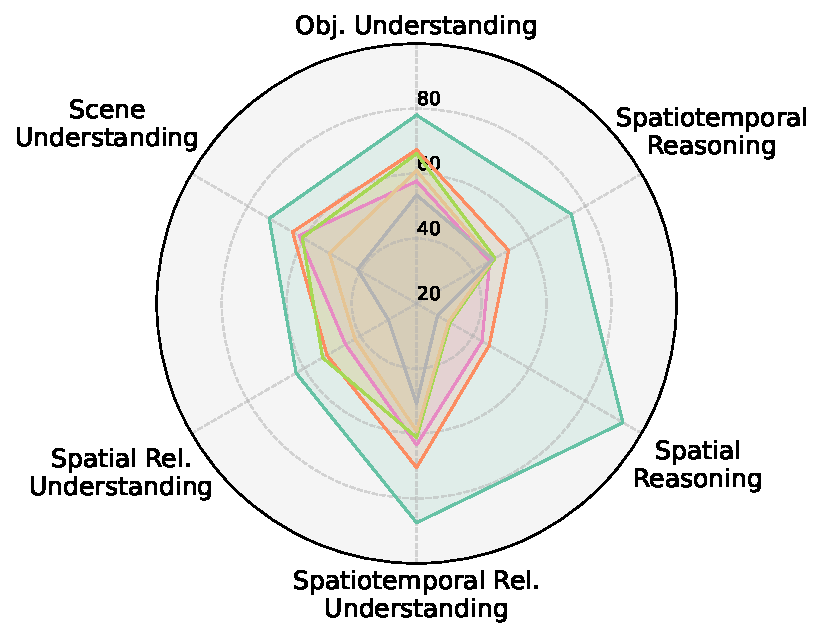
\includegraphics[width=\linewidth]{Figures/results_all_v2.pdf}
        \caption{All categories}
        \label{fig:left}
    \end{subfigure}\hfill
    \begin{subfigure}{0.61\textwidth}
        \centering
        \begin{subfigure}[t]{0.32\textwidth}
            \centering
            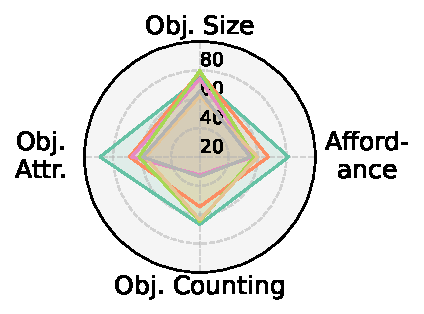
\includegraphics[width=\linewidth]{Figures/results_object_understanding_v2.pdf}
            \vspace{-1.75em}
            \captionsetup{font=scriptsize}
            \caption{Obj. Understanding}
            \label{fig:1b}
        \end{subfigure}\hfill
        \begin{subfigure}[t]{0.32\textwidth}
            \centering
            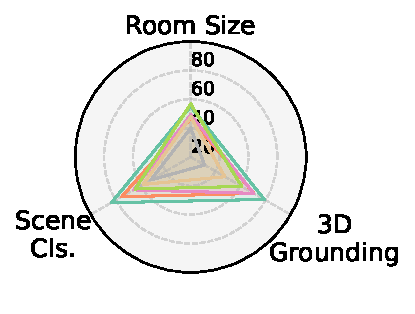
\includegraphics[width=\linewidth]{Figures/results_scene_understanding_v2.pdf}
            \vspace{-1.75em}
            \captionsetup{font=scriptsize}
            \caption{Scene Understanding}
            \label{fig:1c}
        \end{subfigure}\hfill
        \begin{subfigure}[t]{0.32\textwidth}
            \centering
            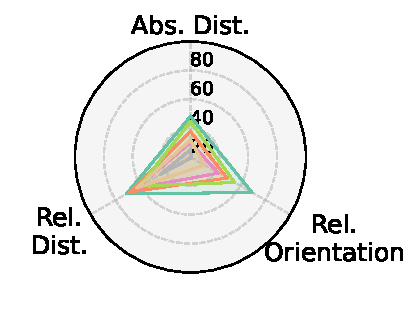
\includegraphics[width=\linewidth]{Figures/results_spatial_v2.pdf}
            \vspace{-1.75em}
            \captionsetup{font=scriptsize}
            \caption{Spatial Rel. Understanding}
            \label{fig:2a}
        \end{subfigure}
        \begin{subfigure}[t]{0.32\textwidth}
            \centering
            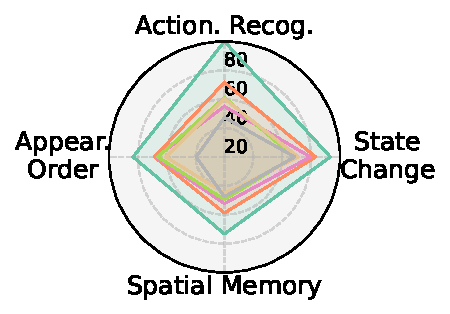
\includegraphics[width=\linewidth]{Figures/results_spatiotemporal_v2.pdf}
            \vspace{-1.75em}
            \captionsetup{
                font=scriptsize,
                justification=centering,
                singlelinecheck=false
            }
            \caption{Spatiotemporal Rel.\\Understanding}
            \label{fig:2b}
        \end{subfigure}\hfill
        \begin{subfigure}[t]{0.32\textwidth}
            \centering
            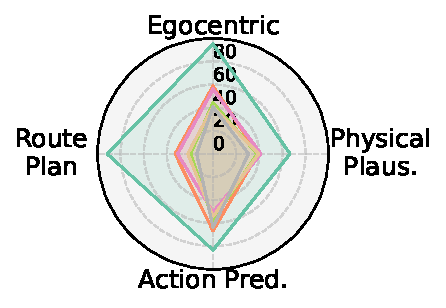
\includegraphics[width=\linewidth]{Figures/results_reasoning_v2.pdf}
            \vspace{-1.75em}
            \captionsetup{
                font=scriptsize,
                justification=centering,
                singlelinecheck=false
            }
            \caption{Spatial \& Spatio-\\temporal Reasoning}
            \label{fig:2c}
        \end{subfigure}\hfill
        \begin{subfigure}[t]{0.32\textwidth}
            \centering
            \vspace{-5em}
            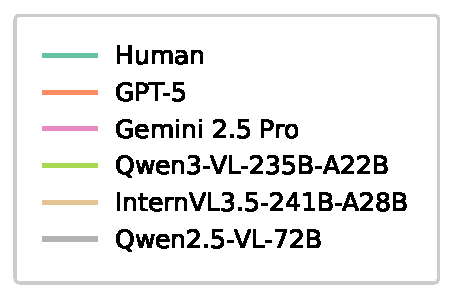
\includegraphics[width=0.8\linewidth]{Figures/results_legend_v2.pdf}
        \end{subfigure}
        \vspace{-0.5em}
    \end{subfigure}
	\caption{Radar chart visualization of model performance across 18 tasks on Spatial4D-Bench.
    }
    \label{Main_results_radar_plot}
\end{figure}







\paragraph{The overall performance gap between MLLMs and human-level 4D spatial intelligence remains significant.}
From~\cref{table:main_eval_18_tasks} and \cref{fig:left}, we can see that the overall 4D spatial intelligence performance of MLLMs remains significantly inferior to that of humans.
The best proprietary model, GPT-5, achieves an average score of $60.90$, while the best open-source model, Qwen3-VL-235B-A22B, yields an average score of $56.17$.
This indicates that the performance gap between the best proprietary MLLMs and the best open-source MLLMs is relatively small, although the best proprietary MLLMs still perform better.
However, the overall performance gap between MLLMs (both proprietary and open-source) and human-level 4D spatial intelligence remains significant.
On Spatial4D-Bench, humans achieve an average score of $78.02$, outperforming the best proprietary model (GPT-5) by approximately $17$ and the best open-source model (Qwen3-VL-235B-A22B) by $22$.
Current MLLMs appear to operate as ``frame-based observers'' rather than ``world observers''.
They lack an intuitive physics engine or coherent temporal memory, preventing effective reasoning about causality, permanence, and dynamics.
Spatial4D-Bench effectively exposes this 4D reasoning gap, which was invisible in existing benchmarks.
Substantial efforts are required to further improve MLLMs toward human-level spatial cognition.
  


\paragraph{MLLMs have reached or even surpassed human-level spatial cognition on some understanding-related tasks.}
As shown in \cref{table:main_eval_18_tasks}, \cref{fig:1b} and \cref{fig:1c}, for the fundamental \textit{object/scene understanding} category (\eg~ \textit{object size}, \textit{object counting}, and \textit{room size}), existing MLLMs often reach or even surpass human performance.
In particular, Qwen3-VL-30B-A3B achieves $80.10$ on the object size estimation task, outperforming the human baseline of $74.61$.
In addition, on the \textit{object counting} task, the best MLLM also outperforms human performance. We attribute this to distinct cognitive processing differences. 
First, while humans rely on intuitive relative scale, they struggle with precise absolute metric estimation (e.g., ``is this table 1.2m or 1.4m?'') from 2D projections without explicit reference scales while MLLMs leverage massive prior knowledge obtained by pre-training on 3D and geometric data which are useful. Moreover, it is noticed that \textit{external factors} can also result in low accuracy of the human evaluation. For example, in \textit{object counting}, to elevate the the difficulty level in model evaluation, Spatial4D-Bench includes a set of low-resolution videos with significant jittering and inconsistent frames compared with videos used in~\cite{Yang_2025_CVPR}, posing a huge challenge to human evaluators in correctly matching and identifying the objects within these videos. We have also found that discrepancies among humans in defining the object categories also play an important role in the low accuracy of this task. While a \textit{nightstand} is considered to be a \textit{table} in the QA design, a human evaluator may not count it as a \textit{table}, causing inconsistent result with the ground truth answer.

\paragraph{MLLMs usually perform significantly worse than humans on spatial reasoning and spatiotemporal reasoning tasks.} The primary source of the human-AI gap lies in reasoning-related tasks.
As shown in \cref{table:main_eval_18_tasks}, \cref{fig:2b}, and \cref{fig:2c}, MLLMs exhibit substantial performance degradation on the \textit{spatial reasoning} and \textit{spatiotemporal reasoning} categories.
These challenging categories are the core of Spatial4D-Bench.
Specifically, for \textit{spatiotemporal reasoning}, even the top-tier MLLMs lag significantly behind humans (e.g., GPT-5 scores $32.83$ on \textit{route plan} vs.\ Human $91.67$).
This \textasciitilde$60\%$ gap highlights a fundamental deficiency of MLLMs in maintaining a coherent 4D world model over extended temporal sequences.
For the \textit{physical plausibility reasoning} task, MLLMs score near random chance ($30\%-40\%$), whereas humans intuitively reject these physically impossible scenarios ($66.67\%$).
This indicates that SOTA MLLMs struggle to ground visual perception in fundamental physical laws.




\begin{table}
\centering
\footnotesize
\begin{tabular}{c@{\extracolsep{4pt}}lcr@{\extracolsep{3pt}}lcr@{\extracolsep{3pt}}lcr@{\extracolsep{3pt}}l}
\toprule
 &  & \multicolumn{3}{c}{\textbf{Qwen3-VL {\tiny 30B-A3B}}} & \multicolumn{3}{c}{\textbf{InternVL3.5 {\tiny 38B}}} & \multicolumn{3}{c}{\textbf{InternVL3.5 {\tiny 8B}}} \\ 
 \cmidrule(lr){3-5} \cmidrule(lr){6-8} \cmidrule(lr){9-11}
 & \multirow{-2}{*}{\textbf{Task}} & \textbf{\scriptsize VSI} & \multicolumn{2}{c}{\textbf{\scriptsize Ours {\tiny ($\Delta$)}}} & \textbf{\scriptsize VSI} & \multicolumn{2}{c}{\textbf{\scriptsize Ours {\tiny ($\Delta$)}}} & \textbf{\scriptsize VSI} & \multicolumn{2}{c}{\textbf{\scriptsize Ours {\tiny ($\Delta$)}}} \\ \midrule
\multirow{4}{*}{\rotatebox[origin=c]{90}{\scriptsize \textit{Numerical}}} & Room Size & 65.17 & 67.22 & {\color{ForestGreen} (+2.05)} & 55.35 & 55.02 & {\color{BrickRed} (-0.33)} & 55.42 & 50.16 & {\color{BrickRed} (-5.26)} \\
 & Object Size & 77.35 & 80.10 & {\color{ForestGreen} (+2.75)} & 65.31 & 65.63 & {\color{ForestGreen} (+0.32)} & 61.19 & 47.39 & {\color{BrickRed} (-13.80)} \\
 & Object Counting & 71.50 & 67.74 & {\color{BrickRed} (-3.76)} & 65.38 & 60.59 & {\color{BrickRed} (-4.79)} & 61.31 & 55.99 & {\color{BrickRed} (-5.32)} \\
 & Absolute Distance & 42.46 & 42.20 & {\color{BrickRed} (-0.26)} & 31.02 & 28.51 & {\color{BrickRed} (-2.51)} & 34.40 & 25.89 & {\color{BrickRed} (-8.51)} \\ \midrule
\multirow{4}{*}{\rotatebox[origin=c]{90}{\scriptsize\textit{\begin{tabular}{@{}c@{}}Multiple\\-choice\end{tabular}}}} & Relative Distance & 54.93 & 58.11 & {\color{ForestGreen} (+3.18)} & 54.58 & 55.48 & {\color{ForestGreen} (+0.90)} & 50.42 & 48.51 & {\color{BrickRed} (-1.91)} \\
 & Relative Orientation & 58.78 & 53.94 & {\color{BrickRed} (-5.83)} & 60.02 & 52.47 & {\color{BrickRed} (-7.55)} & 44.21 & 40.17 & {\color{BrickRed} (-4.04)} \\
 & Route Plan & 41.75 & 12.00 & {\color{BrickRed} (-29.75)} & 37.63 & 15.50 & {\color{BrickRed} (-22.13)} & 34.02 & 9.83 & {\color{BrickRed} (-24.19)} \\
 & Appearance Order & 64.40 & 61.48 & {\color{BrickRed} (-2.92)} & 63.75 & 54.77 & {\color{BrickRed} (-8.98)} & 54.37 & 50.27 & {\color{BrickRed} (-4.10)} \\ \midrule
 & \textit{Average} & 59.54 & 55.23 & {\color{BrickRed} (-4.32)} & 54.13 & 48.50 & {\color{BrickRed} (-5.63)} & 49.42 & 41.03 & {\color{BrickRed} (-8.39)} \\ \bottomrule
\end{tabular}%

\caption{Comparison with VSI-Bench~\cite{Yang_2025_CVPR} on overlapping tasks.
Overall, state-of-the-art models perform worse on our Spatial4D-Bench, especially on the redefined \textit{route plan} task.
These results indicate that our Spatial4D-Bench is more challenging than VSI-Bench~\cite{Yang_2025_CVPR} on overlapping tasks.
}
\label{table:vsi_calib}
\end{table}



\subsection{Benchmark Challenge Analysis}
As summarized in~\cref{tab:recent_mllm_eval_benchmarks}, Spatial4D-Bench provides a more comprehensive evaluation benchmarks with 18 tasks.
Since there are some tasks overlapping with existing benchmarks, it would be interesting to investigate the challenge of these tasks between existing benchmarks and Spatial4D-Bench.
To this end, we compare with VSI-Bench~\cite{Yang_2025_CVPR}, one of the most representative spatial intelligence benchmarks, on overlapping tasks using Qwen3-VL-30B-A3B, InternVL3.5-38B, and InternVL3.5-8B.
As shown in~\cref{table:vsi_calib}, overall, state-of-the-art models perform worse on our Spatial4D-Bench.
Specifically, on some perception-related tasks, \eg, \textit{object size} and \textit{room size}, the performance is comparable across both benchmarks.
However, for more challenging reasoning tasks, such as \textit{relative orientation} and \textit{route plan}, substantial divergences can be observed, especially on the \textit{route plan} task, where the tested models exhibit a substantial performance drop of approximately 22\% to 29\% on Spatial4D-Bench compared to VSI-Bench~\cite{Yang_2025_CVPR}.
In addition to the difficulty elevation described in \cref{subsec:taxonomy}, this can be attributed to the fact that the \textit{route plan} task in Spatial4D-Bench requires long-horizon planning and 4D spatial understanding over longer sequences and more complex state transitions, which distinguishes Spatial4D-Bench from existing benchmarks that may rely on shorter horizons or simpler topological graphs.




\subsection{Further Analysis and Discussion}



\paragraph{Temporal Context and Spatial Memory.}
\textit{Spatial memory} in long video represents a frontier of 4D spatial intelligence, assessing the ability of a model to maintain consistent visual state representations over extended durations.
To study the impact of the sequence length, we evaluate Qwen3-VL-30B-A3B on videos of varying lengths ($5$, $10$, and $30$ minutes).
The evaluated subset comprises $420$, $426$, and $200$ QA pairs for the respective durations, totaling $1,046$ samples.
\begin{wraptable}{r}{0.4\textwidth}
    \centering
    \begin{tabular}{llll}	 
    \toprule 
         \textbf{Video duration}     & \textbf{Accuracy (\%)$\uparrow$} \\         
         \midrule
         5 min     & 0.5381 \\
         10 min    & 0.4343 \\
         30 min    & 0.4250 \\   
    \bottomrule    
	\end{tabular}
    \caption{Impact of video duration on \textit{spatial memory} accuracy (Qwen3-VL-30B-A3B). Performance degrades on longer sequences, highlighting the limitation of fixed-frame sampling in capturing high-frequency spatial updates.}
    \label{table:spatial_memory_video_length}
\end{wraptable}
We present the results in \cref{table:spatial_memory_video_length}.
As expected, performance drops as the video length increases, indicating that the information retrieval architecture can play an important role in the model's reasoning capability, as unified sampling scheme in longer videos will cause more information loss. However, the gap between 10-minute and 30-minute videos is much closer than that between 5-minute and 10 minute videos. We explain it as the bottleneck saturation from temporal aliasing in sampled frames, and the strong language prior will compensate for the information loss from visual input as will be shown later in \cref{table:visual_ablation}. Nonetheless, the result still indicates that solving 4D spatial intelligence requires a paradigm shift from fixed-context windows to adaptive sampling or streaming memory architectures.




\begin{table}[]
\centering
\footnotesize
\begin{tabular}{llcr@{\extracolsep{3pt}}lr@{\extracolsep{3pt}}lc}
\toprule
\textbf{Category} & \textbf{Task} & \textbf{Video Input} & \multicolumn{2}{c}{\textbf{Image Input {\tiny($\Delta$)}}} & \multicolumn{2}{c}{\textbf{Text Input {\tiny($\Delta$)}}}\\ \midrule
\multirow{4}{*}{Object Understanding} & Object Size & 80.10 & 59.92 & {\color{BrickRed}(-20.18)} & 48.48 & {\color{BrickRed}(-31.62)} \\
 & Object Attribute & 58.92 & 48.63 & {\color{BrickRed}(-10.29)} & \textbf{50.63} & {\color{BrickRed}(-8.29)} \\
 & Object Counting & 67.74 & 20.76 & {\color{BrickRed}(-46.98)} & 1.23 & {\color{BrickRed}(-66.51)} \\ 
 & Affordance & 52.41 & 42.91 & {\color{BrickRed}(-29.50)} & 26.14 & {\color{BrickRed}(-26.27)} \\ \midrule
\multirow{3}{*}{Scene Understanding} & Room Size & 67.22 & 12.28 & {\color{BrickRed}(-54.94)} & \textbf{27.47} & {\color{BrickRed}(-39.75)} \\
& Scene Classification & 54.72 & 36.93 & {\color{BrickRed}(-17.79)} & \textbf{44.62} & {\color{BrickRed}(-10.11)} \\
 & 3D Grounding & 50.55 & 41.54 & {\color{BrickRed}(-9.01)} & \textbf{45.40} & {\color{BrickRed}(-5.15)} \\ \midrule
\multirow{3}{*}{\begin{tabular}[c]{@{}l@{}}Spatial Relationship\\Understanding\end{tabular}} & Absolute Distance & 42.20 & 24.86 & {\color{BrickRed}(-17.34)} & 22.29 & {\color{BrickRed}(-19.91)} \\
 & Relative Distance & 58.11 & 38.50 & {\color{BrickRed}(-19.61)} & 34.01 & {\color{BrickRed}(-24.10)} \\
 & Relative Orientation & 53.94 & 39.11 & {\color{BrickRed}(-13.84)} & 10.80 & {\color{BrickRed}(-42.15)} \\ \midrule
\multirow{4}{*}{\begin{tabular}[c]{@{}l@{}}Spatiotemporal\\ Relationship\\Understanding\end{tabular}} & Action Recognition & 42.95 & 35.10 & {\color{BrickRed}(-7.85)} & 20.38 & {\color{BrickRed}(-22.57)} \\
 & Appearance Order & 61.48 & 29.96 & {\color{BrickRed}(-31.32)} & \textbf{31.36} & {\color{BrickRed}(-30.12)} \\
 & Spatial Memory & 47.42 & 35.66 & {\color{BrickRed}(-11.76)} &  \textbf{37.19} & {\color{BrickRed}(-10.23)} \\
 & State Change & 72.73 & 42.43 & {\color{BrickRed}(-30.30)} & 40.13 & {\color{BrickRed}(-32.60)} \\ \midrule
 \multirow{2}{*}{Spatial Reasoning} 
 & Egocentric Reasoning & 41.90 & 28.40 & {\color{BrickRed}(-13.50)} & 21.20 & {\color{BrickRed}(-20.70)} \\
 & Route Plan & 12.00 & 10.67 & {\color{BrickRed}(-1.33)} & \textbf{13.67} & {\color{ForestGreen}(+1.67)} \\ \midrule
\multirow{2}{*}{\begin{tabular}[l]{@{}l@{}}Spatiotemporal\\Reasoning\end{tabular}} 
 & Action Prediction & 56.46 & 37.14 & {\color{BrickRed}(-19.32)} & \textbf{39.86} & {\color{BrickRed}(-16.60)} \\
 & Physical Plausibility & 38.33 & 28.00 & {\color{BrickRed}(-10.33)} & 23.11 & {\color{BrickRed}(-15.22)} \\ \midrule
 & \textit{Average} & 53.29 & 34.04 & {\color{BrickRed}(-19.24)} & 29.89 & {\color{BrickRed}(-23.40)} \\ \bottomrule
\end{tabular}
\caption{Visual Ablation Study evaluated on Qwen3-VL-30B-A3B. \textbf{Video Input}: Full 64 frames. \textbf{Image Input}: Single frame (random). \textbf{Text Input}: Text-only. While performance generally degrades as visual information is removed, text-only input (bolded) outperforms single-frame input in tasks requiring global context (e.g., \textit{route plan}, \textit{scene classification}), suggesting that incomplete visual data can act as a distractor that overrides correct language priors.}

\label{table:visual_ablation}
\end{table}


\paragraph{Visual Ablation: Disentangling Perception from Language Priors.}
To assess the genuine spatial-temporal reasoning capabilities of MLLMs versus their reliance on language shortcuts, we conduct a visual ablation study on Qwen3-VL-30B-A3B.
We compare the standard \textbf{Video Input} ($64$ frames) against two baselines: \textbf{Single Frame} (a randomly selected image) and \textbf{Text Only} (blind evaluation with no visual input).
The results shown in Table~\ref{table:visual_ablation} reveal distinct performance patterns.

\begin{itemize}
    \item{
        \textbf{The Necessity of 4D Signals.}
        The significant performance gap between video and text-only inputs confirms the validity of Spatial4D-Bench.
        On average, removing visual signals causes a performance drop of $23.40\%$.
        This degradation is most pronounced in dynamic tasks such as \textit{state change} ($-32.60\%$) and \textit{object counting} ($-66.51\%$), demonstrating that these tasks require explicit temporal integration and cannot be solved via language models alone. For example, the model simply outputs $0$ for every question in \textit{object counting} without visual input.
    }
    \item{
        \textbf{The ``Blind'' Leading the ``One-Eyed''.}
        A distinct phenomenon emerges when comparing Text Only vs. Single Frame inputs.
        On eight specific tasks, \ie, \textit{object attribute, room size, scene classification, 3D grounding, appearance order, spatial memory, route plan} and \textit{action prediction}, the blind text-only baseline outperforms the single-frame input.
        For example, on \textit{scene classification}, text-only input achieves $44.62\%$ compared to $36.93\%$ for single-frame.
        We attribute this anomaly to two factors:
        \begin{enumerate}
            \item {\textbf{Language Priors vs.\ Random Chance:}
            In the absence of visual data, the model defaults to learned LLM priors, \eg, probabilistically associating ``oven'' with ``kitchen''.
            As similarly observed on VSI-Bench~\cite{Yang_2025_CVPR}, these priors often provide a statistical floor that is significantly better than random chance.}
            \item \textbf{The ``Misleading Frame'' Hypothesis:}
            For tasks requiring global or temporal continuity (\eg, \textit{room size} and \textit{route plan}), a single random frame often acts as an adversarial distractor.
            If the question concerns an entire apartment but the random frame depicts a small bathroom, the visual signal actively contradicts the correct answer, overriding the model's correct language prior.
        \end{enumerate}
        This inversion highlights a critical limitation in existing MLLMs: they struggle to weigh conflicting evidence, often letting incomplete visual data override reliable language priors.
    }
    \item{
        \textbf{The Route Plan Failure Case.}
        Most alarmingly, providing full video input for \textit{route plan} yields negligible improvement over the blind baseline (12.00\% vs 13.67\%).
        This suggests that current MLLMs struggle to construct a coherent spatial map from egocentric videos, effectively reverting to random guessing or language priors even when visual data are provided.
    }
\end{itemize}



\begin{figure}[t!]
	\centering	
	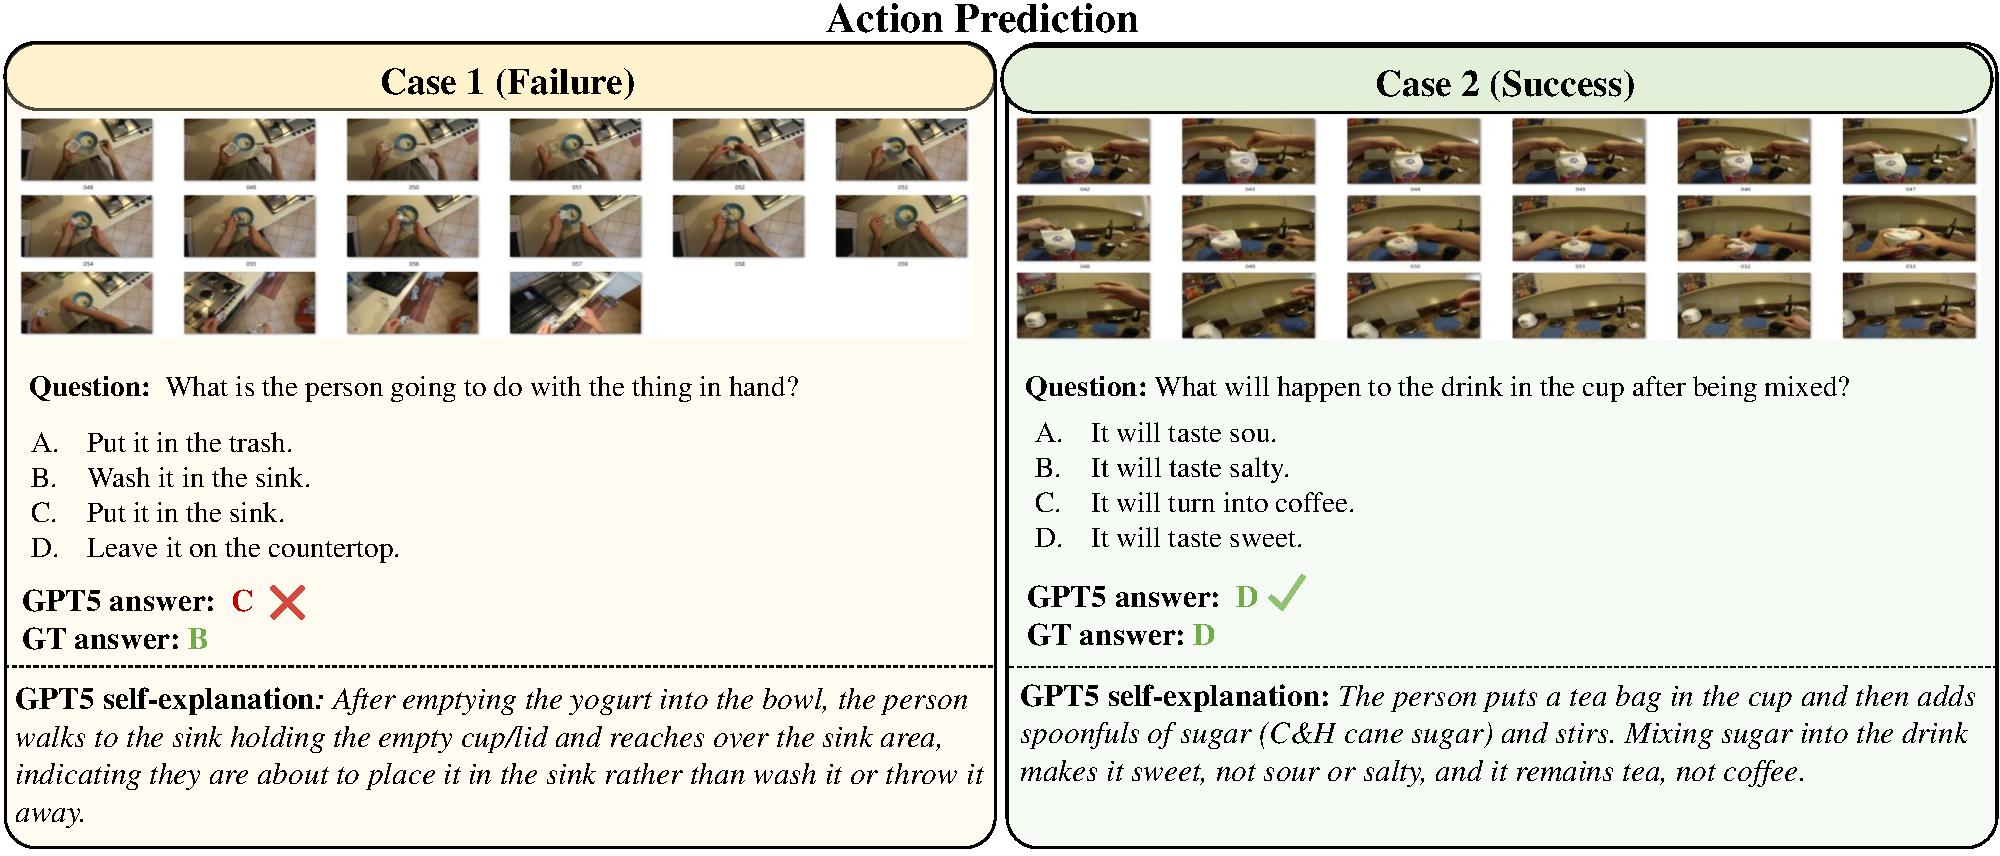
\includegraphics[width=\columnwidth]{Figures/failure_cases/GPT5_Action_Prediction.pdf} 		
	\caption{Action prediction examples (GPT-5). Spatial4D-Bench exposes the conflict between general semantic priors and specific visual evidence (Case 1), while validating successful text-driven reasoning (Case 2).
	\label{GPT5_spatial_time_causal_prediction_examples} }
\end{figure}

\subsection{Qualitative Case Analysis}
\label{sec:failure_analysis}

Our Spatial4D-Bench has exposed the critical bottlenecks of state-of-the-art MLLMs, especially on \textit{spatial reasoning} and \textit{spatiotemporal reasoning}.
However, quantitative metrics often mask the underlying reasoning processes. To uncover \textit{why} models fail, we analyze the failure and success cases of GPT-5, the top-performing MLLM on our evaluation, and leverage its self-explanation capabilities to trace the precise reasoning pathways that lead to errors.
In this way, we showcase how Spatial4D-Bench successfully exposes the systemic bottlenecks of MLLMs in maintaining temporal coherence, physical grounding, and perceptual fidelity that remain hidden in existing spatial intelligence benchmarks.






\paragraph{MLLMs are Relatively Fragile in Spatiotemporal Continuity.}
A major challenge in 4D spatial intelligence is \textit{spatiotemporal reasoning} that requires understanding a coherent 4D world over time rather than treating videos as a collection of disjoint semantic concepts.
By designing tasks that connect past, present, and future visual observations, Spatial4D-Bench reveals a significant \textit{temporal incoherence} in SOTA MLLMs.
\cref{GPT5_spatial_time_causal_prediction_examples} shows failure and success cases from the \textit{action prediction} task, which exposes this fragility.
In \textbf{Case 1} (failure), the ground truth action is ``washing'' a yogurt cup, but the model incorrectly predicts ``placing it in the sink'', driven by a semantic prior rather than the specific temporal action.
The benchmark's design allows us to probe the cause via the model's self-explanation: \textit{``...the person walks to the sink holding the empty cup... indicating they are about to place it in the sink rather than wash it or throw it away''}.
This textual feedback from the model demonstrates that the model successfully tracked the trajectory but failed to infer the latent intent (washing for recycling), proving that even powerful models fail to ground their predictions in the actual temporal dynamics when those dynamics conflict with training priors.
On the other hand, \textbf{Case 2} (success) validates the benchmark's ability to measure robust chain-of-thought reasoning when explicit cues (OCR) are present.
The model correctly infers the drink will taste ``sweet'' by synthesizing the label ``sugar'' with the stirring action (\textit{``mixing sugar into the drink makes it sweet...''}).
This contrast underscores the diagnostic value of our Spatial4D-Bench: it can distinguish between scenarios where models rely on robust textual grounding versus those where they collapse into hallucination due to temporal ambiguity.



\begin{figure}[t]
	\centering	
	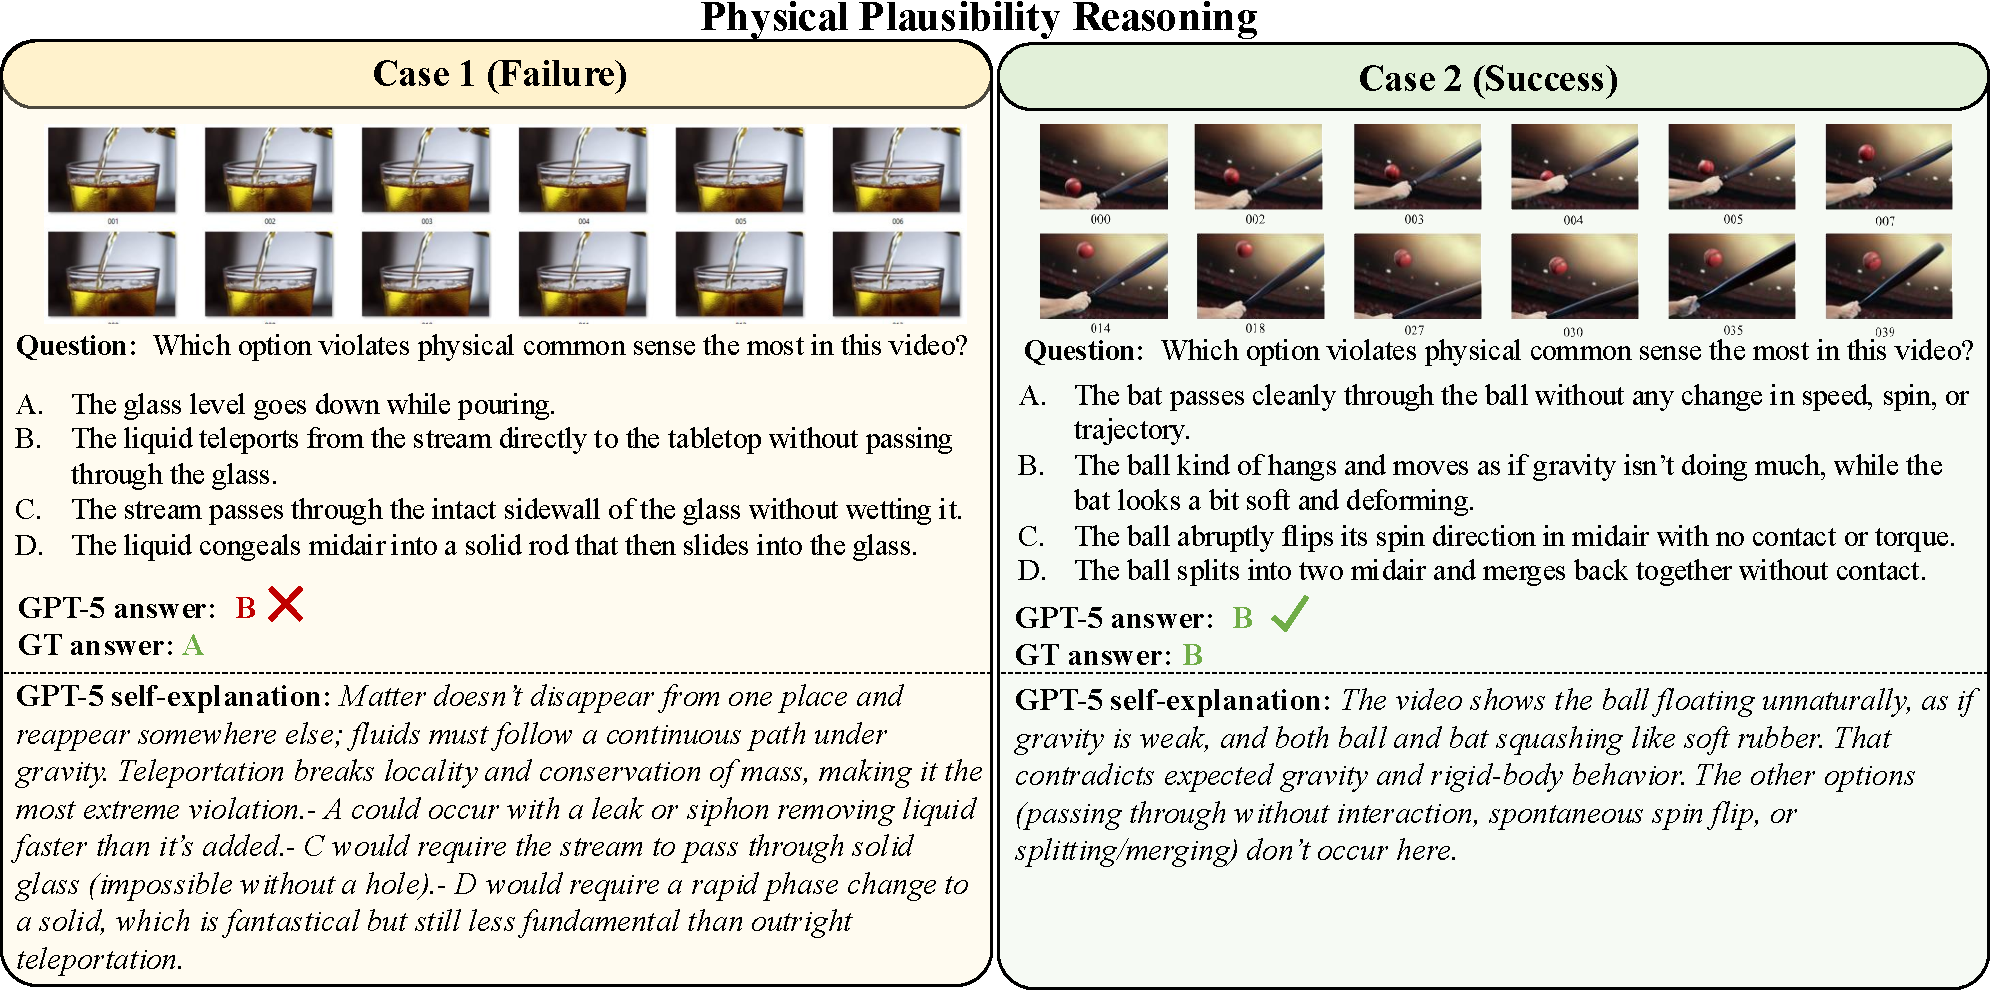
\includegraphics[width=\columnwidth]{Figures/failure_cases/GPT5_Physical_Plausibility_Reasoning.pdf}
	\caption{Physical plausibility reasoning examples (GPT-5). Spatial4D-Bench reveals that models can hallucinate physical justifications (Case 1) despite possessing correct theoretical knowledge, highlighting the gap between semantic and visual understanding.
	\label{GPT5_physical_common_sense_examples} }
\end{figure}

\paragraph{MLLMs Exhibit a Knowledge-Perception Gap in Intuitive Physics.}
By incorporating the \textit{physical plausibility reasoning} in the \textit{spatiotemporal reasoning} category, specifically using AI-generated physical anomalies, Spatial4D-Bench provides a unique evaluation of the ``intuitive physics engine'' of MLLMs.
Our evaluation exposes a sharp dissociation between low-level perceptual grounding and high-level physical knowledge.
In \cref{GPT5_physical_common_sense_examples} \textbf{Case 1} (failure), the benchmark challenges the model with a subtle violation of fluid dynamics.
GPT-5 fails to identify a physical anomaly where liquid levels behave inconsistently during pouring, yet its self-explanation recites perfect high-level physics principles: \textit{``Matter doesn’t disappear from one place and reappear somewhere else... Teleportation breaks locality and conservation of mass...''}.
This result highlights a critical insight enabled by our benchmark: SOTA models possess abstract knowledge of physical laws but lack the visual grounding to detect their violation in pixel space.
The model ``knows'' the laws of physics but cannot ``see'' them being broken, relying instead on analyzing the textual plausibility of the options (e.g., rejecting ``teleportation'' as a concept) rather than verifying the visual dynamics.
Spatial4D-Bench thus serves as a necessary filter to differentiate between models that merely \textit{know} physics textually and those that can \textit{perceive} physics visually.
In contrast, \textbf{Case 2} (success) shows that the model is capable of detecting violations in rigid body dynamics. It correctly identifies that a baseball and bat exhibit unnatural softness and defy gravity, suggesting that conspicuous deviations in material properties and trajectory dynamics are easier for current architectures to flag than subtle fluid inconsistencies.

\begin{figure}[t]
	\centering	
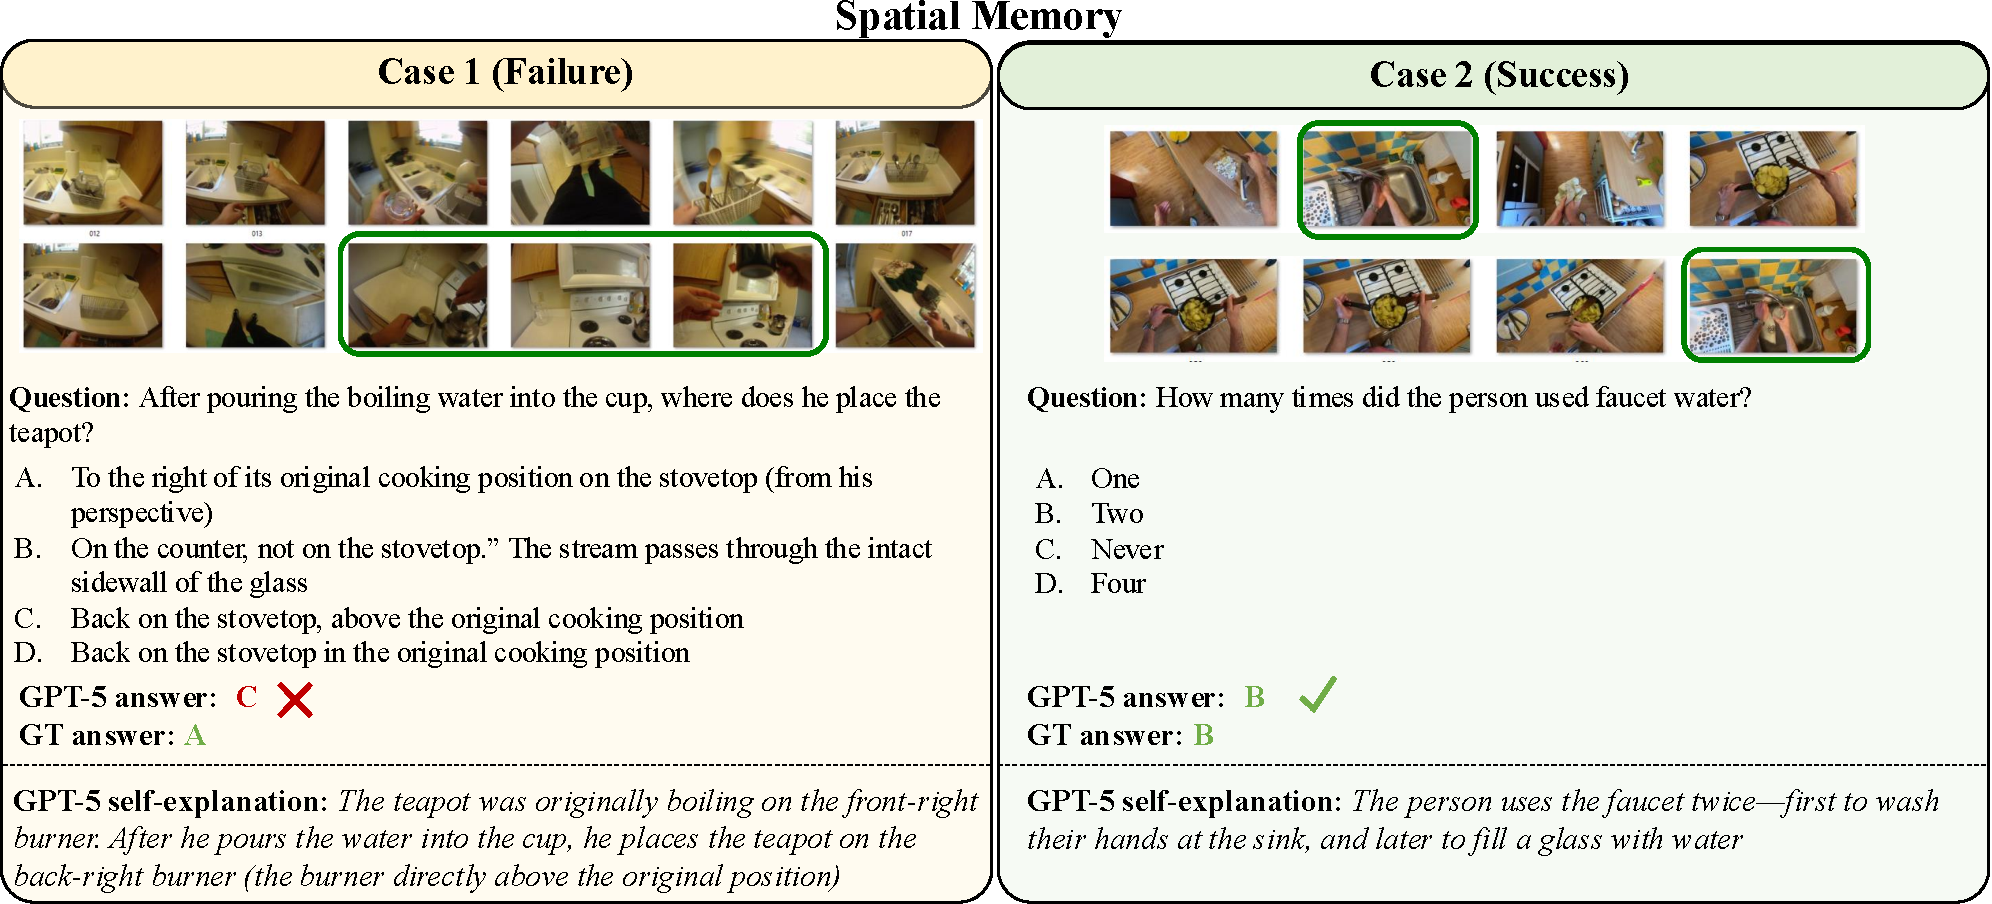
\includegraphics[width=\columnwidth]{Figures/failure_cases/GPT5_spatial_memory.pdf} 		
	\caption{The benchmark's fine-grained tracking requirements expose confident hallucinations driven by texture confusion (Case 1).
	\label{GPT5_spatial_memory_failure_examples} }
\end{figure}


\begin{figure}[t]
	\centering	
	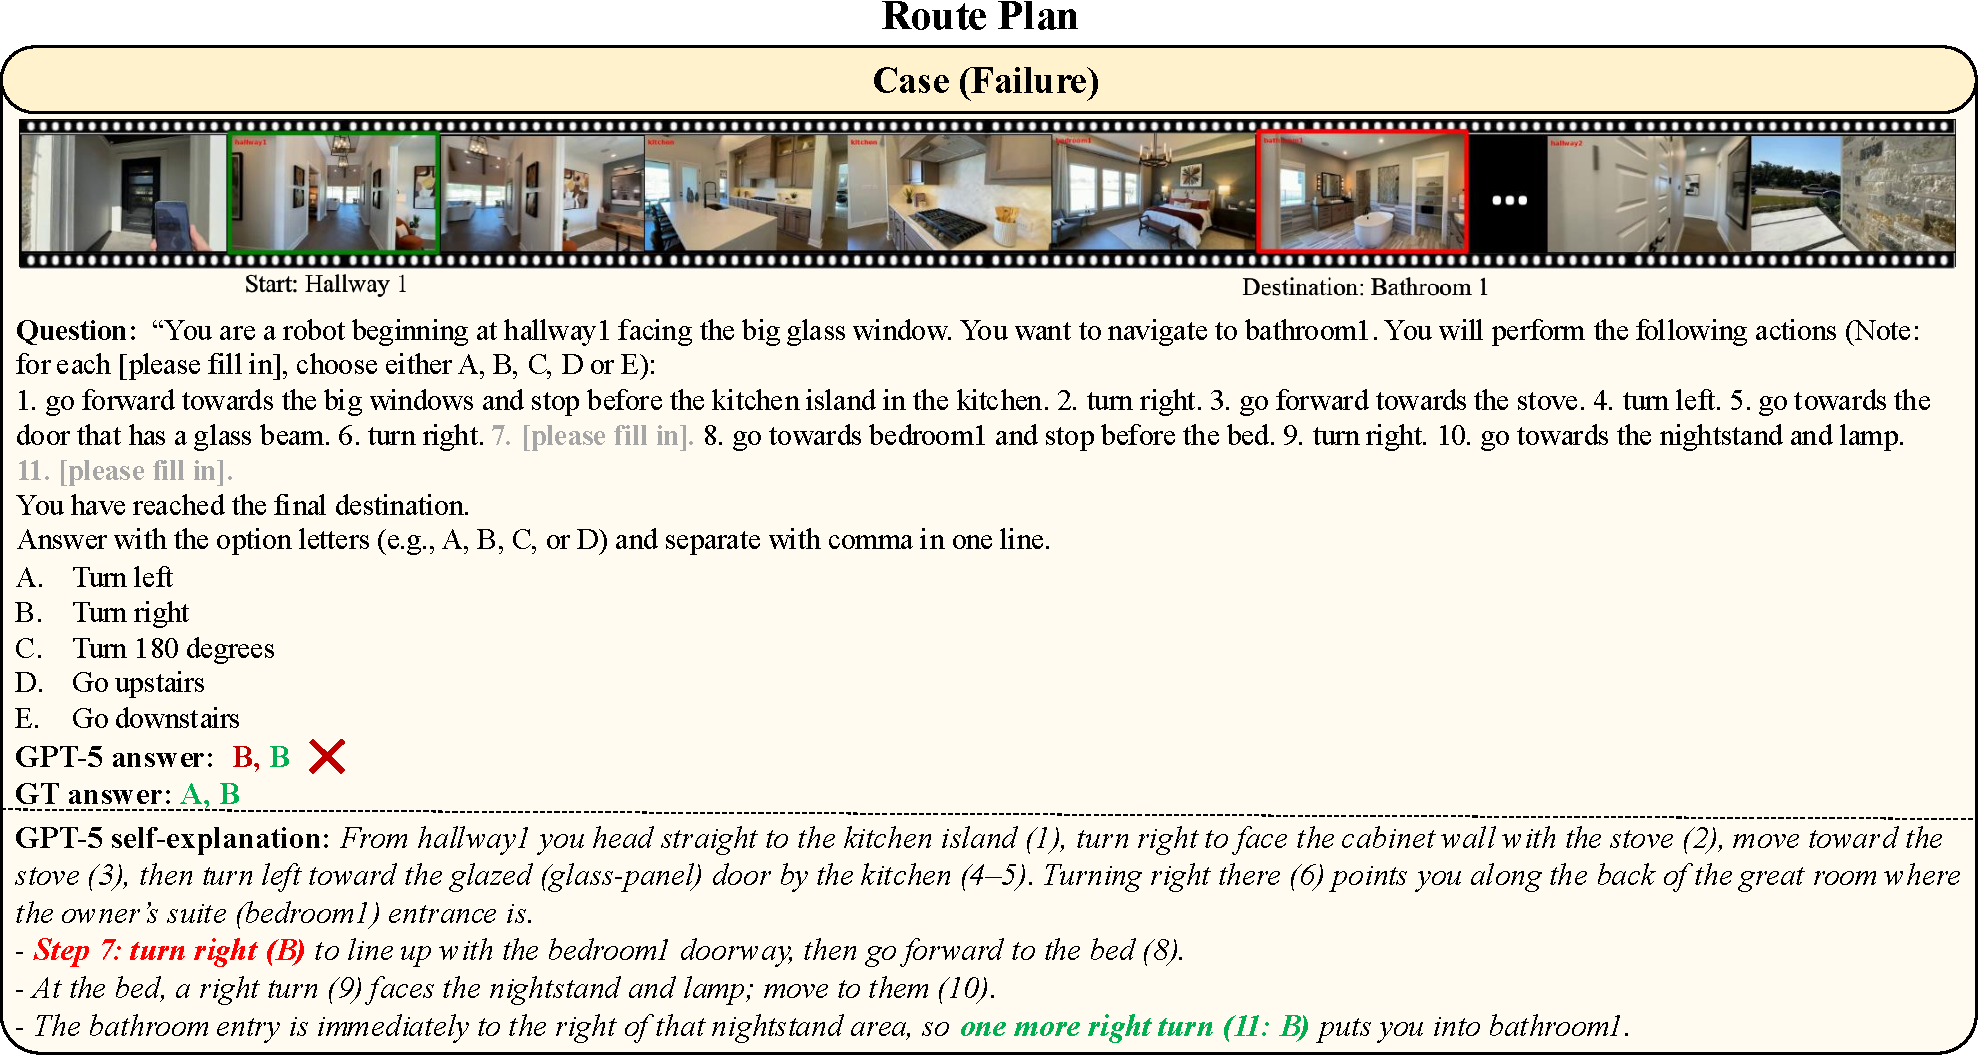
\includegraphics[width=\columnwidth]{Figures/failure_cases/GPT5_navigation.pdf}	
    \caption{Route plan failure case (GPT-5). 
    The model attempts to plan a path from the hallway to the bathroom but fails to ground its reasoning in the scene's geometry. 
    At step 7, the model confidently justifies a right turn (option B) to enter the bedroom, hallucinating a spatial layout that fits its internal narrative. 
    However, the visual evidence dictates a left turn (option A) is required to face the doorway. 
    This illustrates a critical limitation where SOTA models fail to maintain visual spatial consistency in long-horizon planning.}
	\label{fig:GPT5_navigation_failure} 
\end{figure}

\paragraph{MLLMs have Spatial Hallucination Driven by Texture Confusion.}
Through evaluation on Spatial4D-Bench, we observe that perceptual ambiguity can lead to confident hallucinations, even in tasks (such as \textit{spatial memory}) that require explicit tracking.
In \cref{GPT5_spatial_memory_failure_examples} \textbf{Case 1} (failure), the model incorrectly localizes the final position of a teapot. 
Crucially, the self-explanation reveals a confident hallucination: \textit{``After he pours the water... he places the teapot on the back-right burner (the burner directly above the original position)''}.
This contradicts the visual evidence of the teapot's placement in other locations.
This suggests that texture similarity across the stove top surface causes the model to lose track of the object's specific geometric coordinates.
Unlike a tracking failure where a model might express uncertainty, here the model constructs a coherent (but false) narrative to fill the perceptual gap.
This failure mode validates the necessity of Spatial4D-Bench's fine-grained annotation: unlike simpler existence or classification tasks, our spatial memory queries force the model to confront texture confusion and occlusion.
The benchmark demonstrates that even when a model is confident and generates plausible-sounding narratives, it often lacks the precise metric grounding required for 4D spatial intelligence.
By contrast, \textbf{Case 2} (success) demonstrates that the model maintains robust temporal tracking when visual events are semantically distinct.
The model correctly counts that the faucet was used ``two'' times.
Its self-explanation, \textit{``...first to wash their hands at the sink, and later to fill a glass with water''}, shows a successful linking of two separate temporal events, implying that the ``grounding gap'' is highly sensitive to visual saliency.
The model fails when tracking requires resolving low-level texture ambiguity (Case 1) but succeeds when tracking high-level, semantically distinct actions (Case 2), further validating the benchmark's ability to probe the granular limits of spatial memory.




\paragraph{MLLMs Rely on Hallucination in Egocentric Route Plan.}
The \textit{route plan} task in the \textit{spatial reasoning} category illustrates the inability of current MLLMs to construct accurate mental maps from egocentric video streams. 
In \cref{fig:GPT5_navigation_failure}, the model attempts to plan a path from a hallway to a bathroom. 
While GPT-5 outputs a confident self-explanation, reasoning that a right turn at step 7 would ``line up with the bedroom doorway'', this contradicts the visual geometry: the robot has just entered a hallway configuration where a left turn (option A) is geometrically required to face the bedroom entrance. 
The model hallucinates a spatial layout that fits its internal narrative but ignores the visual reality of the scene. 
Furthermore, while the model correctly identifies the final turn (step 11) as a right turn, this success is coincidental, derived from a flawed intermediate trajectory. 
This failure highlights a critical bottleneck: SOTA MLLMs struggle with long-horizon spatial consistency and relative orientation. 
By enforcing strict directional accuracy over multi-step paths, Spatial4D-Bench effectively disentangles true embodied route planning capabilities from lucky guesses driven by language priors.

